\documentclass{article}
\usepackage[utf8]{inputenc}

\usepackage{amsmath}
\usepackage{amsfonts}
\usepackage{pifont}
\usepackage{times}
\usepackage{sectsty}

\usepackage[top=2cm, bottom=1cm, left=2cm, right=2cm]{geometry}                 

\title{Surface Curvature Distributions as Biomarkers of Dyslexia}
\author{Rudolph Pienaar}
\date{}

\usepackage{natbib}
\usepackage{graphicx}

\begin{document}

\maketitle

\abstract

This is the abstract

\section{Introduction}

First paragraph, what we are trying to do. How, and why.

Second group: what is currently done

Third group: Why is this new, important?

Fourth group: Paper layout/overview

\section{Methods}

Patient groups, number, how collected and initially processed.

Curvature analysis.

\section{Results}

\begin{figure}[h!]
\centering
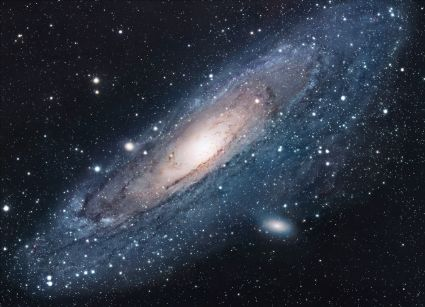
\includegraphics[scale=1.7]{fig-1.jpg}
\caption{The Universe}
\label{threadsVsSync}
\end{figure}

\section{Discussion}


\section{Conclusion}

\bibliographystyle{plain}
\bibliography{references}
\end{document}

